\documentclass[unicode,14pt]{beamer}
\usepackage{mypresentation}
\usetikzlibrary{positioning,calc}

% for makein
\definecolor{blizzardblue}{rgb}{0.67, 0.9, 0.93}
\definecolor{bleudefrance}{rgb}{0.19, 0.55, 0.91}

\protected\def\pdfliteral{\pdfextension literal}
\newcommand{\TikZ}{Ti\textit{k}Z}

\def\coloredtitle{}
\title{文字の一部に色を塗る}
\author{\sffamily 鹿野 桂一郎\\
\bfseries ラムダノート株式会社\\
\small\bfseries \email{k16.shikano@lambdanote.com} \\ 
\twitter{golden\_lucky} 
}
\date{\sffamily\footnotesize 2024年11月30日\\ 於\, TeXConf 2024}

\begin{document}

\frame{\titlepage}

\setbeamertemplate{background canvas}[vertical shading][bottom=white,top=kachi!15]
\setbeamercolor{frametitle}{bg=kachi, fg=white}
\setbeamercolor{structure}{fg=kachi}

\begin{frame}[t]{\inhibitglue 目次}
  \sffamily
  \begin{itemize}
    \item 文字の色は均一であることが多い
    \item 1文字が複数の色で塗り分けられる場合
    \item 実装編(装飾的タイポグラフィ)
  \end{itemize}
\end{frame}

\begin{frame}[t]{文字の色は均一であることが多い}
  \sffamily
  \begin{itemize}
    \item 情報伝達の手段なので
    \item 書記体系におけるアトミックな要素なので
    \item 刷版と印刷の都合
  \end{itemize}
  \begin{center}
    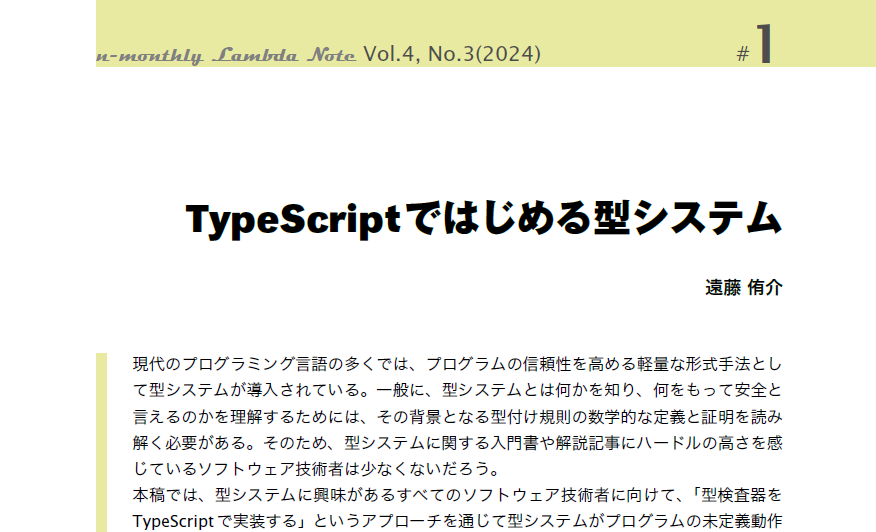
\includegraphics[width=.50\textwidth]{figures/nlambda.png}
  \end{center}
\raggedleft\tiny\color{50gray} 『n月刊ラムダノート Vol.4, No.3』 ラムダノート 2024
\end{frame}

\setbeamertemplate{background canvas}[vertical shading][bottom=white,top=miru!15]
\setbeamercolor{frametitle}{bg=miru, fg=white}
\setbeamercolor{structure}{fg=miru}

\begin{frame}[t]{1文字が複数の色で塗り分けられる場合}
  \sffamily
  \begin{itemize}
\item レタリング
\item 装飾頭文字
\item 装飾的タイポグラフィ
\item ワードアート(的なもの)
\item カラー絵文字
  \end{itemize}
\end{frame}

\begin{frame}[t]{レタリング}
  \sffamily
  \begin{itemize}
\item 一文字ずつ手作業で描かれた絵としての文字
  \end{itemize}
  \begin{center}
    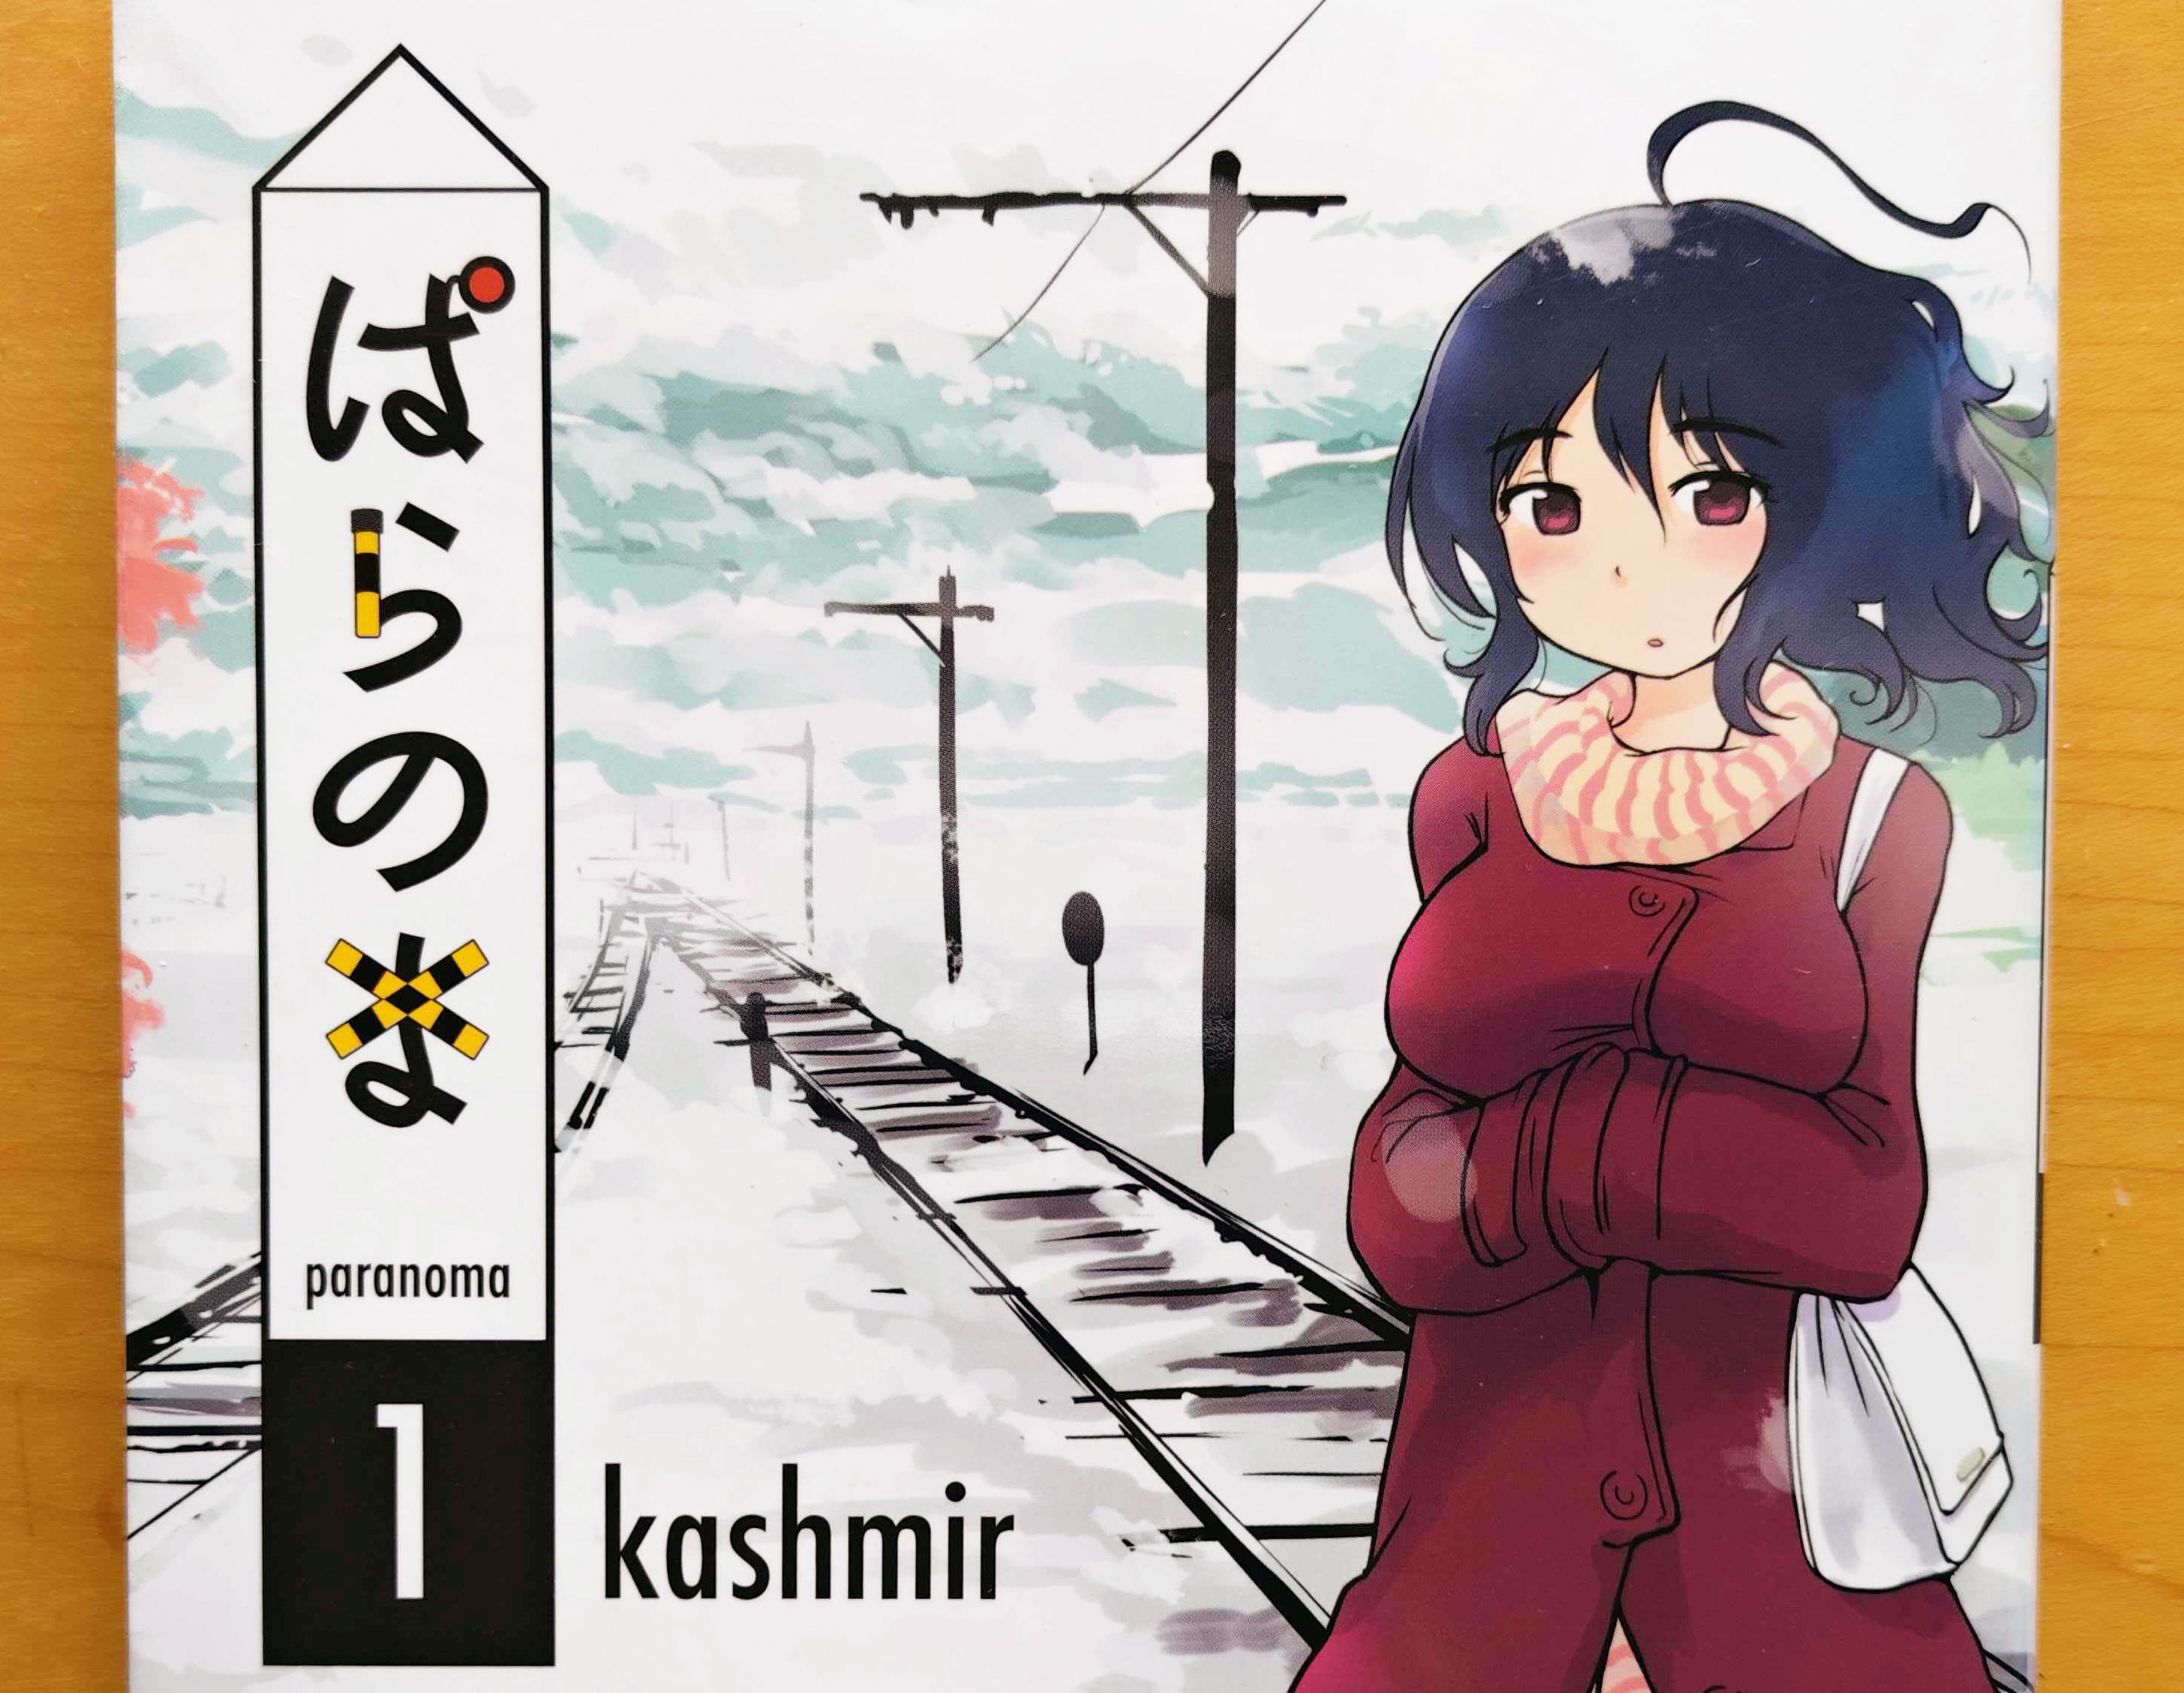
\includegraphics[width=.50\textwidth]{figures/paranoma.jpg}
  \end{center}
\raggedleft\tiny\color{50gray} kashimr 『ぱらのま1』 白泉社 2017
\end{frame}

\begin{frame}[t]{装飾頭文字}
  \sffamily
  \begin{itemize}
\item ドロップキャップとかで使われる華美な文字
\item レタリングに似ているが現代ではフォントにもなっている
  \end{itemize}
  \begin{center}
    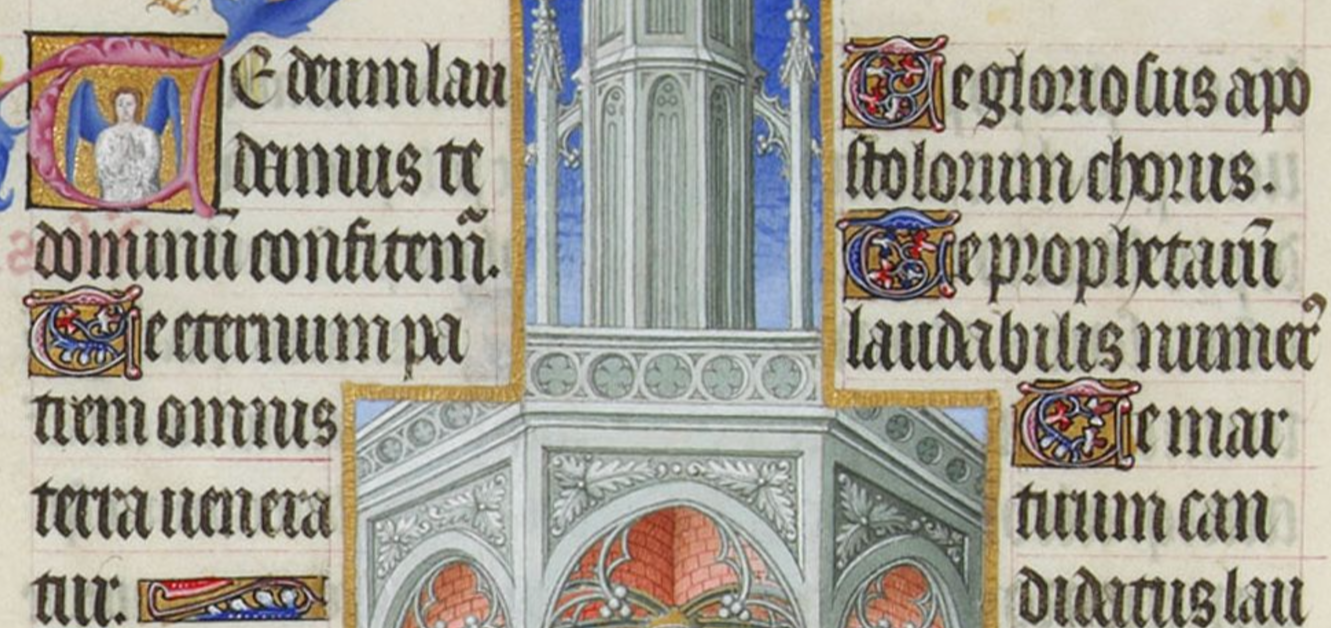
\includegraphics[width=.50\textwidth]{figures/Folio_37v.png}
  \end{center}
\raggedleft\tiny\color{50gray} 『ベリー公のいとも豪華なる時祷書 聖アウグスティヌスの洗礼』 15世紀\par
\url{https://commons.wikimedia.org/wiki/File:Folio_37v_-_The_Baptism_of_Saint_Augustine.jpg}
\end{frame}

\begin{frame}[t]{装飾的タイポグラフィ1}
  \sffamily
  \begin{itemize}
\item フォントを利用して文字に装飾を施す
  \end{itemize}
  \begin{center}
    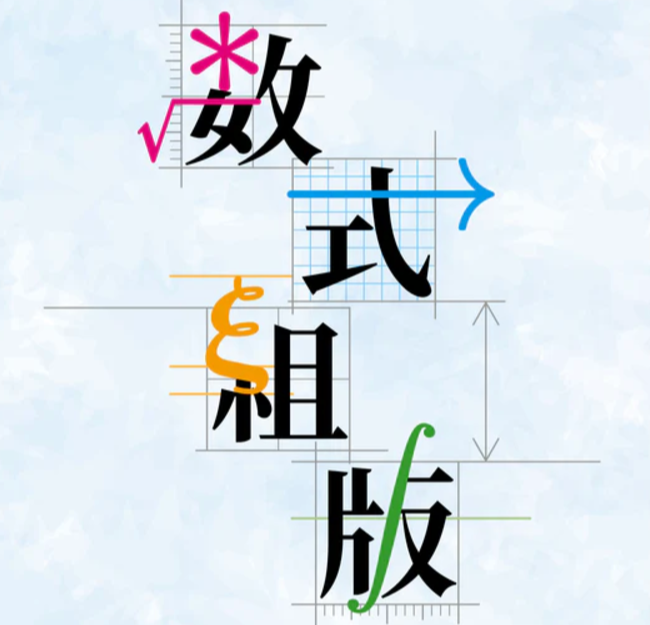
\includegraphics[width=.40\textwidth]{figures/sushiki-kumihan.png}
  \end{center}
\raggedleft\tiny\color{50gray} 木枝祐介 『数式組版』 ラムダノート 2018
\end{frame}

\begin{frame}[t]{装飾的タイポグラフィ2}
  \sffamily
  \begin{itemize}
\item フォントを利用して文字に装飾を施す
  \end{itemize}
  \begin{center}
    
\includegraphics[width=.65\textwidth]{figures/makein.png}
  \end{center}
\raggedleft\tiny\color{50gray} 
『負けヒロインが多すぎる!』2024年版アニメオープニングより
\end{frame}

\begin{frame}[t]{ワードアート}
  \sffamily
  \begin{itemize}
\item テンプレートを使って手軽に文字を装飾
\item 手軽な反面、制限も多い
\item 例は省略
  \end{itemize}
\end{frame}

\begin{frame}[t]{カラー絵文字}
  \sffamily
  \begin{itemize}
\item OpenTypeやTrueTypeの機能で、グリフ自体に色を付けられる
\item COLRテーブルとCPALテーブルを使う
\item OpenType 1.9(2021年)以降はCOLRv1テーブル
\item OpenType-SVGというのもある
  \end{itemize}
  \begin{center}
    
\includegraphics[width=.5\textwidth]{figures/emoji.png}
  \end{center}
\end{frame}

\setbeamertemplate{background canvas}[vertical shading][bottom=white,top=yamabuki!15]
\setbeamercolor{frametitle}{bg=yamabuki, fg=black}
\setbeamercolor{structure}{fg=yamabuki}

\begin{frame}[plain]
  \begin{center}
    \HUGE{34}{34}\color{black}
    実装編\par
    \HUGE{23}{23}\color{50gray}
    (装飾的タイポグラフィ)
  \end{center}
\end{frame}

\begin{frame}[t]{グリフのパスをクリップして背景を描画}
  \sffamily
  \begin{itemize}
  \item PostScriptでよく知られている方法
  \end{itemize}
  \begin{columns}[t]
    \begin{column}{.35\textwidth}
  \begin{enumerate}
\item グリフのパスをクリップする
\item 色①で領域を塗り潰す
\item 色②で領域を塗り潰す
  \end{enumerate}
    \end{column}
    \begin{column}{.6\textwidth}
  \begin{center}
    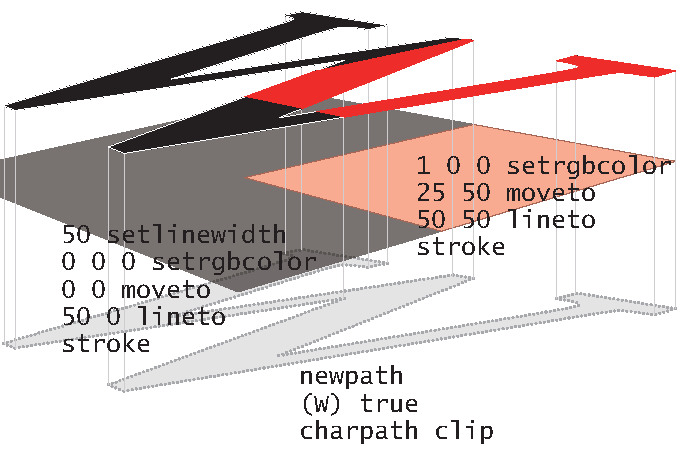
\includegraphics[width=\textwidth]{figures/w-clip-ps.pdf}
    \vfill
  \end{center}
    \end{column}
  \end{columns}
\end{frame}

\begin{frame}[fragile]{グリフのパスをクリップして背景を描画}
  \sffamily
  \vspace*{-\baselineskip}
  \begin{columns}[t]
    \begin{column}{.5\textwidth}
  \begin{tcolorbox}[sharp corners]
  \HUGE{8}{9}
  \begin{Verbatim}[commandchars=\\\{\}, breaklines=true, breakanywhere=true]
\KeywordTok{newpath}
\DecValTok{0} \DecValTok{0} \KeywordTok{moveto}
\StringTok{(W)} \KeywordTok{true}
\KeywordTok{charpath} \KeywordTok{clip}

\DecValTok{50} \KeywordTok{setlinewidth}
\DecValTok{0} \DecValTok{0} \DecValTok{0} \KeywordTok{setrgbcolor}
\DecValTok{0} \DecValTok{0} \KeywordTok{moveto}
\DecValTok{50} \DecValTok{0} \KeywordTok{lineto}
\KeywordTok{stroke}

\DecValTok{1} \DecValTok{0} \DecValTok{0} \KeywordTok{setrgbcolor}
\DecValTok{25} \DecValTok{50} \KeywordTok{moveto}
\DecValTok{50} \DecValTok{50} \KeywordTok{lineto}
\KeywordTok{stroke}
  \end{Verbatim}
  \end{tcolorbox}
    \end{column}
    \begin{column}{.5\textwidth}
  \begin{center}
    \mbox{}
    \vfill
    
\includegraphics[width=.75\textwidth]{figures/wclip-ps.pdf}
    \vfill
  \end{center}
    \end{column}
  \end{columns}
\end{frame}

\begin{frame}[t]{グリフのパスをクリップして背景を描画}
  \sffamily
  \begin{itemize}
\item Illustratorではもちろん使える
\item CSSでも使える
  \begin{itemize}
  \item \texttt{background-clip: text;}
  \item \texttt{background-image: linear-gradient(...)}
  \end{itemize}  
\item MS Wordにはそもそもワードアートしかない(が、ワードアートも原理は同じ)
\item PDFには該当の命令がない(\texttt{W}命令でクリップできるのはグラフィックのみ)
  \end{itemize}
\end{frame}

\begin{frame}[t]{\TikZ{}による実現方法}
  \sffamily
  \begin{columns}[t]
    \begin{column}{.4\textwidth}
  \begin{enumerate}
\item 色①で文字を書く
\item その文字の範囲のうち、「色②にしたい領域を切り出すパス」を書いて、\texttt{\textbackslash{}clip}する
\item 同じ座標に色②で文字を書く
  \end{enumerate}
    \end{column}
    \begin{column}{.6\textwidth}
  \begin{center}
    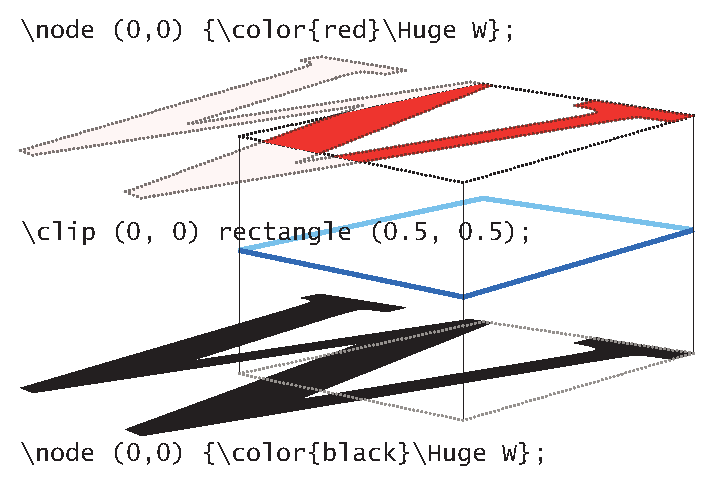
\includegraphics[width=\textwidth]{figures/w-clip.pdf}
  \end{center}
    \end{column}
  \end{columns}
\end{frame}

\begin{frame}[fragile]{\TikZ{}による実現方法}
  \sffamily
  \vspace*{-\baselineskip}
  \begin{columns}[t]
    \begin{column}{.55\textwidth}
  \begin{tcolorbox}[sharp corners]
  \HUGE{8}{9}
  \begin{Verbatim}[commandchars=\\\{\}, breaklines=true, breakanywhere=true]
\BuiltInTok{\textbackslash{}documentclass}\NormalTok{\{}\ExtensionTok{standalone}\NormalTok{\}}
\BuiltInTok{\textbackslash{}usepackage}\NormalTok{\{}\ExtensionTok{tikz}\NormalTok{\}}
\KeywordTok{\textbackslash{}begin}\NormalTok{\{}\ExtensionTok{document}\NormalTok{\}}

\KeywordTok{\textbackslash{}begin}\NormalTok{\{}\ExtensionTok{tikzpicture}\NormalTok{\}}
  \FunctionTok{\textbackslash{}node}\NormalTok{ (0,0) }
    \NormalTok{\{}\FunctionTok{\textbackslash{}color}\NormalTok{\{black\}}\FunctionTok{\textbackslash{}bfseries}\NormalTok{ W\};}
  \FunctionTok{\textbackslash{}clip}\NormalTok{ (0, 0) }
    \NormalTok{rectangle (0.5, 0.5);}
  \FunctionTok{\textbackslash{}node}\NormalTok{ (0,0) }
    \NormalTok{\{}\FunctionTok{\textbackslash{}color}\NormalTok{\{red\}}\FunctionTok{\textbackslash{}bfseries}\NormalTok{ W\};}
\KeywordTok{\textbackslash{}end}\NormalTok{\{}\ExtensionTok{tikzpicture}\NormalTok{\}}

\KeywordTok{\textbackslash{}end}\NormalTok{\{}\ExtensionTok{document}\NormalTok{\}}
  \end{Verbatim}
  \end{tcolorbox}
    \end{column}
    \begin{column}{.45\textwidth}
  \begin{center}
    \mbox{}
    \vfill
    
\includegraphics[width=.85\textwidth]{figures/wclip.pdf}
    \vfill
  \end{center}
    \end{column}
  \end{columns}
\end{frame}


\begin{frame}[fragile]{ちょっと楽しくなってきた}
  \sffamily
  \vspace*{-\baselineskip}
  \begin{tcolorbox}[sharp corners]
  \HUGE{4.5pt}{6pt}
  \begin{Verbatim}[commandchars=\\\{\}, breaklines=true, breakanywhere=true]
\BuiltInTok{\textbackslash{}documentclass}\NormalTok{[lualatex]\{}\ExtensionTok{jlreq}\NormalTok{\}}
\BuiltInTok{\textbackslash{}usepackage}\NormalTok{[haranoaji,deluxe]\{}\ExtensionTok{luatexja{-}preset}\NormalTok{\}}
\BuiltInTok{\textbackslash{}usepackage}\NormalTok{\{}\ExtensionTok{tikz}\NormalTok{\}}
\FunctionTok{\textbackslash{}usetikzlibrary}\NormalTok{\{positioning,calc\}}

\BuiltInTok{\textbackslash{}usepackage}\NormalTok{\{}\ExtensionTok{xcolor}\NormalTok{\}}
\FunctionTok{\textbackslash{}definecolor}\NormalTok{\{blizzardblue\}\{rgb\}\{0.67, 0.9, 0.93\}}
\FunctionTok{\textbackslash{}definecolor}\NormalTok{\{bleudefrance\}\{rgb\}\{0.19, 0.55, 0.91\}}
\KeywordTok{\textbackslash{}begin}\NormalTok{\{}\ExtensionTok{document}\NormalTok{\}}

\KeywordTok{\textbackslash{}begin}\NormalTok{\{}\ExtensionTok{tikzpicture}\NormalTok{\}}
  \FunctionTok{\textbackslash{}node}\NormalTok{[anchor=base, yshift={-}0.0ex, inner sep=0pt, outer sep=0pt, minimum height=0pt, minimum width=0pt] }
\NormalTok{    (A) at (0,0) }
\NormalTok{    \{}\FunctionTok{\textbackslash{}color}\NormalTok{\{bleudefrance\}}\FunctionTok{\textbackslash{}gtfamily\textbackslash{}bfseries\textbackslash{}fontsize}\NormalTok{\{200px\}\{200px\}}\FunctionTok{\textbackslash{}selectfont}\NormalTok{ 負\};}

  \KeywordTok{\textbackslash{}begin}\NormalTok{\{}\ExtensionTok{scope}\NormalTok{\}}
    \FunctionTok{\textbackslash{}clip}\NormalTok{ [shift=\{(A.south west)\}, xshift=0mm, yshift=0mm] (110px, 90px) rectangle (200px, 155px);}
    \FunctionTok{\textbackslash{}node}\NormalTok{[anchor=base, yshift={-}0.0ex, inner sep=0pt, outer sep=0pt, minimum height=0pt, minimum width=0pt] }
\NormalTok{      (0,0) }
\NormalTok{      \{}\FunctionTok{\textbackslash{}color}\NormalTok{\{blizzardblue\}}\FunctionTok{\textbackslash{}gtfamily\textbackslash{}bfseries\textbackslash{}fontsize}\NormalTok{\{200px\}\{200px\}}\FunctionTok{\textbackslash{}selectfont}\NormalTok{ 負\};}
  \KeywordTok{\textbackslash{}end}\NormalTok{\{}\ExtensionTok{scope}\NormalTok{\}}

  \KeywordTok{\textbackslash{}begin}\NormalTok{\{}\ExtensionTok{scope}\NormalTok{\}}
    \FunctionTok{\textbackslash{}clip}\NormalTok{ [shift=\{(A.south west)\}, xshift=0mm, yshift=0mm] (0px, 0px) rectangle (100px, 39px);}
    \FunctionTok{\textbackslash{}node}\NormalTok{[anchor=base, yshift={-}0.0ex, inner sep=0pt, outer sep=0pt, minimum height=0pt, minimum width=0pt] }
\NormalTok{      (0,0) }
\NormalTok{      \{}\FunctionTok{\textbackslash{}color}\NormalTok{\{blizzardblue\}}\FunctionTok{\textbackslash{}gtfamily\textbackslash{}bfseries\textbackslash{}fontsize}\NormalTok{\{200px\}\{200px\}}\FunctionTok{\textbackslash{}selectfont}\NormalTok{ 負\};}
  \KeywordTok{\textbackslash{}end}\NormalTok{\{}\ExtensionTok{scope}\NormalTok{\}}
\KeywordTok{\textbackslash{}end}\NormalTok{\{}\ExtensionTok{tikzpicture}\NormalTok{\}}

\KeywordTok{\textbackslash{}end}\NormalTok{\{}\ExtensionTok{document}\NormalTok{\}}
  \end{Verbatim}
  \end{tcolorbox}
\end{frame}

\begin{frame}[t]{ちょっと楽しくなってきた}
\begin{center}
\begin{tikzpicture}
  \node[anchor=base, yshift=-0.0ex, inner sep=0pt, outer sep=0pt, minimum height=0pt, minimum width=0pt] 
    (A) at (0,0) 
    {\color{bleudefrance}\gtfamily\bfseries\fontsize{200px}{200px}\selectfont 負};

  \begin{scope}
    \clip [shift={(A.south west)}, xshift=0mm, yshift=0mm] (110px, 90px) rectangle (200px, 155px);
    \node[anchor=base, yshift=-0.0ex, inner sep=0pt, outer sep=0pt, minimum height=0pt, minimum width=0pt] 
      (0,0) 
      {\color{blizzardblue}\gtfamily\bfseries\fontsize{200px}{200px}\selectfont 負};
  \end{scope}

  \begin{scope}
    \clip [shift={(A.south west)}, xshift=0mm, yshift=0mm] (0px, 0px) rectangle (100px, 39px);
    \node[anchor=base, yshift=-0.0ex, inner sep=0pt, outer sep=0pt, minimum height=0pt, minimum width=0pt] 
      (0,0) 
      {\color{blizzardblue}\gtfamily\bfseries\fontsize{200px}{200px}\selectfont 負};
  \end{scope}
\end{tikzpicture}
\end{center}
\end{frame}

\begin{frame}[t]{装飾的タイポグラフィ2(再掲)}
  \sffamily
  \begin{itemize}
\item フォントを利用して文字に装飾を施す
  \end{itemize}
  \begin{center}
    
\includegraphics[width=.65\textwidth]{figures/makein.png}
  \end{center}
\raggedleft\tiny\color{50gray} 
『負けヒロインが多すぎる!』2024年版アニメオープニングより
\end{frame}

\begin{frame}[t]{漢字のパーツに色が塗られている!}
  \sffamily
  \begin{center}
    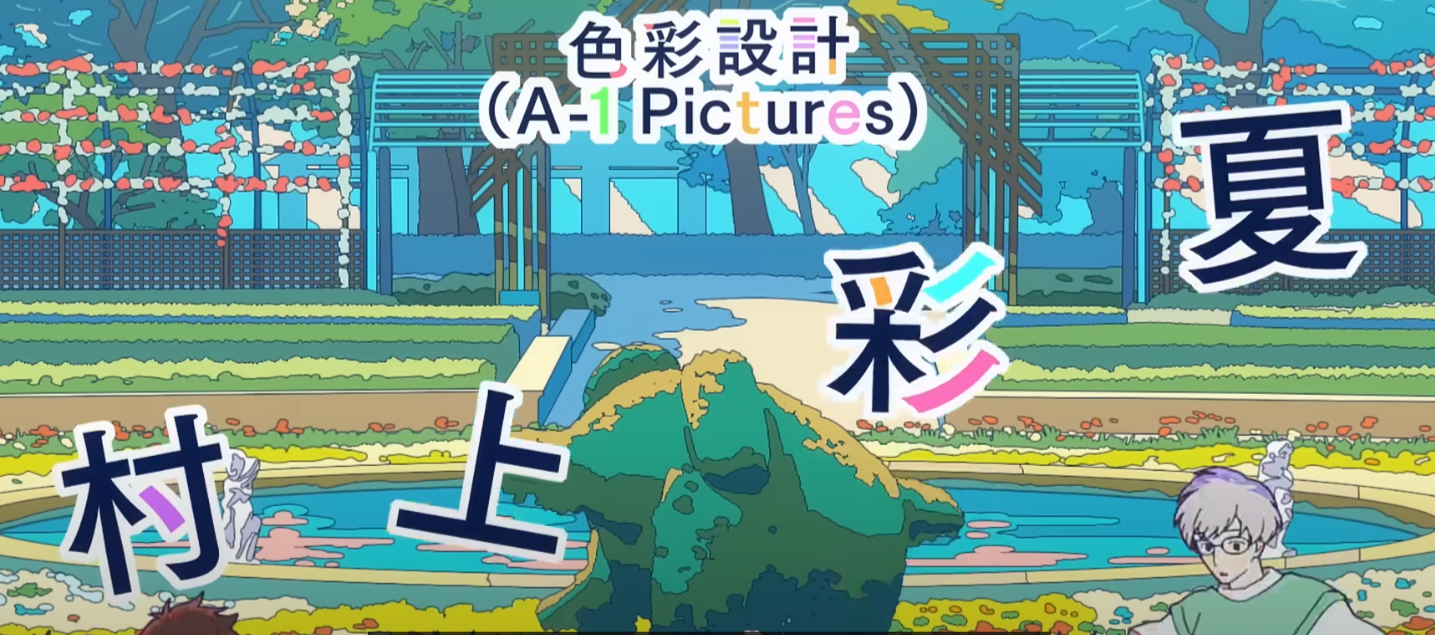
\includegraphics[width=.65\textwidth]{figures/makein2.png}
  \end{center}
\raggedleft\tiny\color{50gray} 
『負けヒロインが多すぎる!』2024年版アニメオープニングより 
\end{frame}

\begin{frame}[t]{漢字のパーツのパスを手に入れる}
  \sffamily
  \begin{itemize}
\item 漢字のパーツのパスさえ手に入れば原理的に可能
\item グリフをレンダリングして、その結果をOpenCVで画像解析して各パーツの輪郭を抽出し、他のパーツが重なってる部分を除去
\item コードは略(ChatGPTに書かせればいいので)
  \end{itemize}
  \begin{center}
    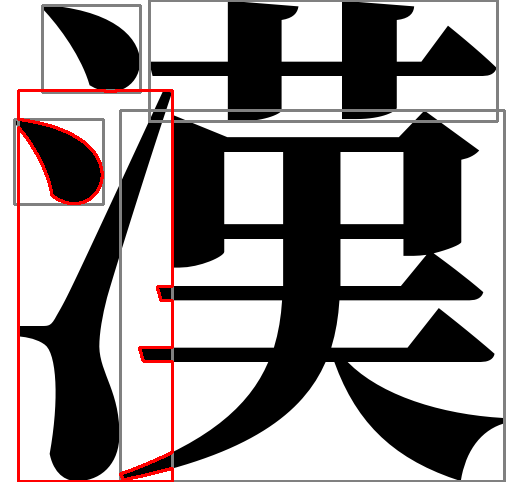
\includegraphics[width=.3\textwidth]{figures/segmented_glyph_with_polygon.png}
  \end{center}
\end{frame}


\begin{frame}[t]{ちょっと「版ズレ」してるけど文字}
\begin{center}

% beamerのせいか、200ptのフォントサイズを指定しても微妙に小さくなってしまうので、PDFでフォントを実測して逆算して207.78ptとしている
% yshiftにも謎の補正-7ptが必要
% いずれもふつうの文書クラスでは不要
\begin{tikzpicture}
  \node[anchor=base, yshift=-0ex, inner sep=0pt, outer sep=0pt, minimum height=0pt, minimum width=0pt] 
    (A) at (0,0) 
    {\color{black}\rmfamily\bfseries\fontsize{207.78pt}{207.78pt}\selectfont 彩};

  \begin{scope}
\clip [shift={(A.south west)}, xshift=0mm, yshift=207.78pt-7pt, xscale=1, yscale=-1] (0,0) (134.88pt,111.75pt) -- (134.49pt,112.14pt) -- (134.09pt,112.14pt) -- (133.70pt,112.53pt) -- (132.92pt,112.53pt) -- (132.53pt,112.92pt) -- (132.13pt,112.92pt) -- (131.74pt,113.31pt) -- (131.35pt,113.31pt) -- (130.96pt,113.71pt) -- (130.17pt,113.71pt) -- (129.78pt,114.10pt) -- (129.39pt,114.10pt) -- (129.00pt,114.49pt) -- (128.61pt,114.49pt) -- (128.21pt,114.88pt) -- (127.43pt,114.88pt) -- (127.04pt,115.27pt) -- (126.65pt,115.27pt) -- (126.25pt,115.67pt) -- (125.47pt,115.67pt) -- (125.08pt,116.06pt) -- (124.68pt,116.06pt) -- (124.29pt,116.45pt) -- (123.51pt,116.45pt) -- (123.12pt,116.84pt) -- (122.33pt,116.84pt) -- (121.94pt,117.23pt) -- (121.55pt,117.23pt) -- (121.16pt,117.63pt) -- (120.37pt,117.63pt) -- (119.98pt,118.02pt) -- (119.20pt,118.02pt) -- (118.80pt,118.41pt) -- (118.02pt,118.41pt) -- (117.63pt,118.80pt) -- (116.84pt,118.80pt) -- (116.45pt,119.20pt) -- (116.06pt,119.20pt) -- (115.67pt,119.59pt) -- (114.88pt,119.59pt) -- (114.49pt,119.98pt) -- (113.71pt,119.98pt) -- (113.31pt,120.37pt) -- (112.14pt,120.37pt) -- (111.75pt,120.76pt) -- (110.96pt,120.76pt) -- (110.57pt,121.16pt) -- (109.39pt,121.16pt) -- (109.39pt,120.37pt) -- (109.00pt,119.98pt) -- (109.00pt,119.59pt) --
(108.61pt,119.20pt) -- (109.39pt,118.41pt) -- (109.79pt,118.41pt) -- (110.96pt,117.23pt) -- (111.35pt,117.23pt) -- (112.53pt,116.06pt) -- (112.92pt,116.06pt) -- (114.49pt,114.49pt) -- (114.88pt,114.49pt) -- (116.45pt,112.92pt) -- (116.84pt,112.92pt) -- (118.41pt,111.35pt) -- (94.89pt,111.35pt) -- (94.89pt,124.29pt) --
(95.28pt,124.68pt) -- (96.06pt,124.68pt) -- (96.45pt,125.08pt) -- (97.24pt,125.08pt) -- (97.63pt,125.47pt) -- (98.02pt,125.47pt) -- (98.41pt,125.86pt) -- (99.20pt,125.86pt) -- (99.59pt,126.25pt) -- (99.98pt,126.25pt) -- (100.37pt,126.65pt)
-- (100.77pt,126.65pt) -- (101.16pt,127.04pt) -- (101.55pt,127.04pt) -- (101.94pt,127.43pt) -- (102.34pt,127.43pt) -- (102.73pt,127.82pt) -- (103.12pt,127.82pt) -- (103.51pt,128.21pt) -- (103.90pt,128.21pt) -- (104.30pt,128.61pt) -- (104.69pt,128.61pt) -- (105.47pt,129.39pt) -- (105.86pt,129.39pt) -- (106.26pt,129.78pt) -- (106.65pt,129.78pt) -- (107.82pt,130.96pt) -- (108.22pt,130.96pt) -- (109.39pt,132.13pt) -- (109.79pt,132.13pt) -- (112.92pt,135.27pt) -- (112.92pt,135.66pt) -- (114.10pt,136.84pt) -- (114.10pt,137.23pt) -- (114.88pt,138.02pt) -- (114.88pt,138.41pt) -- (115.67pt,139.19pt) -- (115.67pt,139.58pt) -- (116.06pt,139.98pt) -- (116.06pt,140.37pt) -- (116.45pt,140.76pt) -- (116.45pt,141.54pt) -- (116.84pt,141.94pt) -- (116.84pt,142.72pt) -- (117.23pt,143.11pt) -- (117.23pt,144.68pt) -- (117.63pt,145.07pt) -- (117.63pt,149.78pt) -- (117.23pt,150.17pt) -- (117.23pt,151.35pt) -- (116.84pt,151.74pt) -- (116.84pt,152.52pt) -- (116.45pt,152.92pt) -- (116.45pt,153.70pt) -- (116.06pt,154.09pt) -- (116.06pt,154.48pt) -- (115.27pt,155.27pt) -- (115.27pt,155.66pt) -- (114.49pt,156.44pt) -- (114.49pt,156.84pt) -- (112.14pt,159.19pt) -- (111.75pt,159.19pt) -- (110.96pt,159.97pt) -- (110.57pt,159.97pt) -- (110.18pt,160.36pt) -- (109.79pt,160.36pt) -- (109.39pt,160.76pt) -- (109.00pt,160.76pt) -- (108.61pt,161.15pt) -- (107.82pt,161.15pt) --
(107.43pt,161.54pt) -- (106.26pt,161.54pt) -- (105.86pt,161.93pt) -- (101.16pt,161.93pt) -- (100.77pt,161.54pt) -- (99.20pt,161.54pt) -- (98.81pt,161.15pt) -- (98.02pt,161.15pt) -- (97.63pt,160.76pt) -- (97.24pt,160.76pt) -- (96.85pt,160.36pt) -- (96.45pt,160.36pt) -- (96.06pt,159.97pt) -- (95.67pt,159.97pt) -- (95.28pt,159.58pt) -- (94.89pt,159.58pt) -- (94.89pt,196.83pt) -- (199.18pt,196.83pt) -- (199.18pt,111.35pt) -- (136.06pt,111.35pt) -- (135.66pt,111.35pt) -- (135.27pt,111.75pt) -- (134.88pt,111.75pt) -- cycle;
  \node[anchor=base, yshift=-0ex, inner sep=0pt, outer sep=0pt, minimum height=0pt, minimum width=0pt] 
      (0,0) 
    {\color[HTML]{fb6fbd}\rmfamily\bfseries\fontsize{207.78pt}{207.78pt}\selectfont 彩};
  \end{scope}

  \begin{scope}
\clip [shift={(A.south west)}, xshift=0mm, yshift=207.78pt-7pt, xscale=1, yscale=-1] (0,0) (152.92pt,69.40pt) -- (152.92pt,69.01pt) -- (153.31pt,68.62pt) -- (153.31pt,68.22pt) -- (154.09pt,67.44pt) -- (154.09pt,67.05pt) -- (154.48pt,66.66pt) -- (154.48pt,66.26pt) -- (154.88pt,65.87pt) -- (154.88pt,65.48pt) -- (155.66pt,64.69pt) -- (155.66pt,64.30pt) -- (156.05pt,63.91pt) -- (156.05pt,63.52pt) -- (156.44pt,63.13pt) -- (156.44pt,62.73pt) -- (156.84pt,62.34pt) -- (156.84pt,61.95pt) --
(157.23pt,61.56pt) -- (157.23pt,61.17pt) -- (158.01pt,60.38pt) -- (158.01pt,59.99pt) -- (158.40pt,59.60pt) -- (158.40pt,59.21pt) -- (158.80pt,58.81pt) -- (158.80pt,58.42pt) -- (159.19pt,58.03pt) -- (159.19pt,57.64pt) -- (159.58pt,57.25pt) -- (159.58pt,56.85pt) -- (159.97pt,56.46pt) -- (159.97pt,56.07pt) -- (160.36pt,55.68pt) -- (160.36pt,55.28pt) -- (160.76pt,54.89pt) -- (161.15pt,54.89pt) -- (161.54pt,55.28pt) -- (161.93pt,55.28pt) -- (162.33pt,55.68pt) -- (162.72pt,55.68pt) -- (163.11pt,56.07pt) -- (163.50pt,56.07pt) -- (164.29pt,56.85pt) -- (164.68pt,56.85pt) -- (165.07pt,57.25pt) -- (165.46pt,57.25pt) -- (166.25pt,58.03pt) -- (166.64pt,58.03pt) -- (167.03pt,58.42pt) -- (167.42pt,58.42pt) -- (168.21pt,59.21pt) -- (168.60pt,59.21pt) -- (168.99pt,59.60pt) -- (169.38pt,59.60pt) -- (169.77pt,59.99pt) -- (170.17pt,59.99pt) -- (170.95pt,60.77pt) -- (171.34pt,60.77pt) --
(171.74pt,61.17pt) -- (172.13pt,61.17pt) -- (172.91pt,61.95pt) -- (173.30pt,61.95pt) -- (173.70pt,62.34pt) -- (174.09pt,62.34pt) -- (174.87pt,63.13pt) -- (175.26pt,63.13pt) -- (175.66pt,63.52pt) -- (176.05pt,63.52pt) -- (176.44pt,63.91pt) -- (176.83pt,63.91pt) -- (177.62pt,64.69pt) -- (178.01pt,64.69pt) -- (178.40pt,65.09pt) -- (178.79pt,65.09pt) -- (179.58pt,65.87pt) -- (179.97pt,65.87pt) -- (180.36pt,66.26pt) -- (180.75pt,66.26pt) -- (181.54pt,67.05pt) -- (181.93pt,67.05pt) -- (182.32pt,67.44pt) -- (182.71pt,67.44pt) -- (183.11pt,67.83pt) -- (183.50pt,67.83pt) -- (184.28pt,68.62pt) -- (184.67pt,68.62pt) -- (185.07pt,69.01pt) -- (185.46pt,69.01pt) -- (186.24pt,69.79pt) -- (186.63pt,69.79pt) -- (187.03pt,70.18pt) -- (187.42pt,70.18pt) -- (192.91pt,70.18pt) -- (192.91pt,7.45pt) -- (108.61pt,7.45pt) -- (108.61pt,20.00pt) -- (109.39pt,20.78pt) -- (109.79pt,20.78pt) -- (118.41pt,29.41pt) -- (118.80pt,29.41pt) -- (119.20pt,29.80pt) -- (118.41pt,30.58pt) -- (117.63pt,30.58pt) -- (117.23pt,30.98pt) -- (116.45pt,30.98pt) -- (116.06pt,31.37pt) -- (110.96pt,31.37pt) -- (110.57pt,30.98pt) -- (109.00pt,30.98pt) --
(108.61pt,30.58pt) -- (108.61pt,45.87pt) -- (109.00pt,46.27pt) -- (109.79pt,46.27pt) -- (110.18pt,46.66pt) -- (110.57pt,46.66pt) -- (110.96pt,47.05pt) -- (111.75pt,47.05pt) -- (112.14pt,47.44pt) -- (112.53pt,47.44pt) -- (112.92pt,47.83pt) -- (113.71pt,47.83pt) -- (114.10pt,48.23pt) -- (114.49pt,48.23pt) -- (114.88pt,48.62pt) -- (115.27pt,48.62pt) -- (115.67pt,49.01pt) -- (116.45pt,49.01pt) -- (116.84pt,49.40pt) -- (117.23pt,49.40pt) -- (117.63pt,49.80pt) -- (118.41pt,49.80pt) -- (118.80pt,50.19pt) -- (118.80pt,50.58pt) -- (118.41pt,50.97pt) -- (118.41pt,51.36pt) -- (117.63pt,52.15pt) -- (117.23pt,52.15pt) -- (116.45pt,52.93pt) -- (116.06pt,52.93pt) -- (115.67pt,53.32pt) -- (114.49pt,53.32pt) -- (114.10pt,53.72pt) -- (110.96pt,53.72pt) -- (108.61pt,56.07pt) -- (108.61pt,70.18pt) -- (152.13pt,70.18pt) -- (152.92pt,69.40pt) -- cycle;
  \node[anchor=base, yshift=-0ex, inner sep=0pt, outer sep=0pt, minimum height=0pt, minimum width=0pt] 
      (0,0) 
    {\color[HTML]{4afcfc}\rmfamily\bfseries\fontsize{207.78pt}{207.78pt}\selectfont 彩};
  \end{scope}

  \begin{scope}
\clip [shift={(A.south west)}, xshift=0mm, yshift=207.78pt-7pt, xscale=1, yscale=-1] (0,0) (41.17pt,65.87pt) -- (41.17pt,71.75pt) -- (40.78pt,72.14pt) -- (40.78pt,73.32pt) -- (40.78pt,76.85pt) -- (72.14pt,76.85pt) -- (72.14pt,39.99pt) -- (40.78pt,39.99pt) -- (40.78pt,64.30pt) -- (40.78pt,65.48pt) -- (41.17pt,65.87pt) -- cycle;
  \node[anchor=base, yshift=-0ex, inner sep=0pt, outer sep=0pt, minimum height=0pt, minimum width=0pt] 
      (0,0) 
    {\color[HTML]{ffae48}\rmfamily\bfseries\fontsize{207.78pt}{207.78pt}\selectfont 彩};
  \end{scope}
\end{tikzpicture}
\end{center}
\end{frame}

\begin{frame}[t]{文字といえば}
  \vspace*{-2\baselineskip}
  \begin{center}
    \fontsize{207.78pt}{207.78pt}\selectfont ☃
  \end{center}
\end{frame}


\begin{frame}[t]{マフラーのパスを手に入れる}
  \sffamily
  \begin{itemize}
\item 機械学習(画像セグメンテーション)
\item モデルのアーキテクチャはU-Net
\item 誤差関数はDice Loss
\item マフラーありフォントは希少なので、学習用データはaugmentationで補填(合計40サンプル)
\item コードは略(ChatGPTに書かせればいいので)
  \end{itemize}
  \begin{center}
    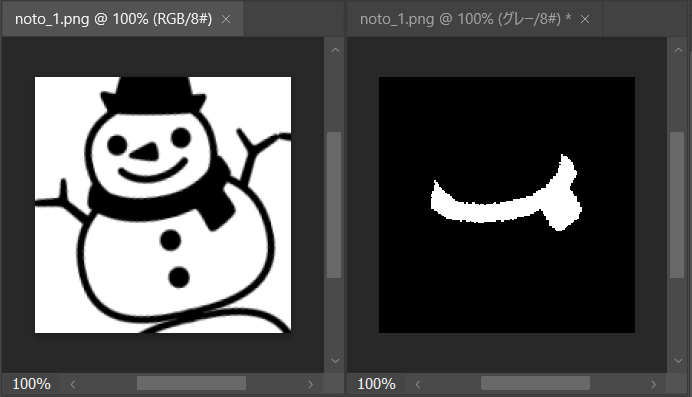
\includegraphics[width=.3\textwidth]{figures/traindata.png}
  \end{center}
\end{frame}


\begin{frame}[t]{画期的}
\begin{center}

% beamerのせいか、200ptのフォントサイズを指定しても微妙に小さくなってしまうので、PDFでフォントを実測して逆算して207.78ptとしている
% yshiftにも謎の補正-7ptが必要
% いずれもふつうの文書クラスでは不要

\begin{tikzpicture}
  \node[anchor=base, yshift=-0ex, inner sep=0pt, outer sep=0pt, minimum height=0pt, minimum width=0pt] 
    (A) at (0,0) 
    {\color{black}\rmfamily\bfseries\fontsize{207.78pt}{207.78pt}\selectfont ☃};
  \begin{scope}
    
\clip [shift={(A.south west)}, xshift=0mm, yshift=207.78pt-7pt, xscale=1, yscale=-1] (0,0) (50.58pt,95.67pt) -- (50.19pt,96.06pt) -- (49.40pt,96.06pt) -- (49.01pt,96.45pt) -- (48.62pt,96.45pt) -- (48.23pt,96.85pt) -- (47.83pt,96.85pt) -- (46.66pt,98.02pt) -- (46.66pt,99.59pt) -- (47.05pt,99.98pt) -- (47.05pt,100.37pt) -- (47.83pt,101.16pt) -- (47.83pt,101.55pt) -- (49.80pt,103.51pt) -- (50.19pt,103.51pt) -- (51.76pt,105.08pt) -- (52.15pt,105.08pt) -- (55.68pt,108.61pt) -- (56.07pt,108.61pt) -- (56.85pt,109.39pt) -- (57.25pt,109.39pt) -- (57.64pt,109.79pt) -- (58.03pt,109.79pt) -- (58.81pt,110.57pt) -- (59.21pt,110.57pt) -- (59.60pt,110.96pt) -- (59.99pt,110.96pt) -- (60.38pt,111.35pt) -- (60.77pt,111.35pt) -- (61.17pt,111.75pt) -- (61.56pt,111.75pt) -- (61.95pt,112.14pt) -- (62.34pt,112.14pt) -- (62.73pt,112.53pt) -- (63.13pt,112.53pt) -- (63.52pt,112.92pt) -- (63.91pt,112.92pt) -- (64.30pt,113.31pt) -- (65.09pt,113.31pt) -- (65.48pt,113.71pt) -- (65.87pt,113.71pt) -- (66.26pt,114.10pt) -- (67.05pt,114.10pt) -- (67.44pt,114.49pt) -- (68.22pt,114.49pt) -- (68.62pt,114.88pt) -- (69.01pt,114.88pt) -- (69.40pt,115.27pt) -- (70.18pt,115.27pt) -- (70.58pt,115.67pt) -- (71.36pt,115.67pt) -- (71.75pt,116.06pt) -- (72.93pt,116.06pt) -- (73.32pt,116.45pt) -- (74.10pt,116.45pt) -- (74.50pt,116.84pt) -- (75.67pt,116.84pt) -- (76.07pt,117.23pt) -- (77.24pt,117.23pt) -- (77.63pt,117.63pt) -- (78.81pt,117.63pt) -- (79.20pt,118.02pt) -- (80.38pt,118.02pt) -- (80.77pt,118.41pt) -- (82.73pt,118.41pt) -- (83.12pt,118.80pt) -- (85.08pt,118.80pt) -- (85.48pt,119.20pt) -- (87.44pt,119.20pt) -- (87.83pt,119.59pt) -- (90.57pt,119.59pt) -- (90.96pt,119.98pt) -- (94.49pt,119.98pt) -- (94.89pt,120.37pt) -- (110.18pt,120.37pt) -- (110.57pt,119.98pt) -- (112.14pt,119.98pt) -- (112.53pt,119.59pt) -- (115.27pt,119.59pt) -- (115.67pt,119.20pt) -- (116.84pt,119.20pt) -- (117.23pt,118.80pt) -- (119.20pt,118.80pt) -- (119.59pt,118.41pt) -- (121.16pt,118.41pt) -- (121.55pt,118.02pt) -- (122.33pt,118.02pt) -- (122.72pt,118.41pt) -- (123.51pt,118.41pt) -- (125.47pt,120.37pt) -- (125.47pt,120.76pt) -- (125.86pt,121.16pt) -- (125.86pt,121.55pt) -- (126.25pt,121.94pt) -- (126.25pt,122.72pt) -- (126.65pt,123.12pt) -- (126.65pt,123.51pt) -- (127.04pt,123.90pt) -- (127.04pt,124.68pt) -- (127.43pt,125.08pt) -- (127.43pt,125.86pt) -- (127.82pt,126.25pt) -- (127.82pt,127.43pt) -- (128.21pt,127.82pt) -- (128.21pt,128.61pt) -- (128.61pt,129.00pt) -- (128.61pt,129.78pt) -- (129.00pt,130.17pt) -- (129.00pt,130.96pt) -- (129.39pt,131.35pt) -- (129.39pt,132.13pt) -- (129.78pt,132.53pt) -- (129.78pt,133.31pt) -- (130.17pt,133.70pt) -- (130.17pt,134.09pt) -- (131.35pt,135.27pt) -- (131.74pt,135.27pt) -- (132.13pt,135.66pt) -- (134.09pt,135.66pt) -- (134.49pt,135.27pt) -- (135.27pt,135.27pt) -- (135.66pt,134.88pt) -- (136.45pt,134.88pt) -- (136.84pt,134.49pt) -- (137.62pt,134.49pt) -- (138.02pt,134.09pt) -- (138.41pt,134.09pt) -- (138.80pt,133.70pt) -- (139.19pt,133.70pt) -- (139.58pt,133.31pt) -- (140.37pt,133.31pt) -- (141.15pt,132.53pt) -- (141.54pt,132.53pt) -- (141.94pt,132.13pt) -- (142.33pt,132.13pt) -- (142.72pt,131.74pt) -- (143.11pt,131.74pt) -- (143.90pt,130.96pt) -- (144.29pt,130.96pt) -- (145.47pt,129.78pt) -- (145.86pt,129.78pt) -- (150.17pt,125.47pt) -- (150.17pt,125.08pt) -- (150.56pt,124.68pt) -- (150.56pt,123.51pt) -- (150.17pt,123.12pt) -- (150.17pt,121.94pt) -- (149.78pt,121.55pt) -- (149.78pt,121.16pt) -- (149.39pt,120.76pt) -- (149.39pt,119.98pt) -- (148.99pt,119.59pt) -- (148.99pt,119.20pt) -- (148.60pt,118.80pt) -- (148.60pt,118.41pt) -- (148.21pt,118.02pt) -- (148.21pt,117.23pt) -- (147.82pt,116.84pt) -- (147.82pt,116.06pt) -- (147.43pt,115.67pt) -- (147.43pt,115.27pt) -- (147.03pt,114.88pt) -- (147.03pt,114.10pt) -- (146.64pt,113.71pt) -- (146.64pt,112.92pt) -- (146.25pt,112.53pt) -- (146.25pt,109.00pt) -- (146.64pt,108.61pt) -- (146.64pt,108.22pt) -- (147.03pt,107.82pt) -- (147.03pt,107.43pt) -- (147.82pt,106.65pt) -- (147.82pt,106.26pt) -- (148.60pt,105.47pt) -- (148.60pt,105.08pt) -- (148.99pt,104.69pt) -- (148.99pt,104.30pt) -- (150.17pt,103.12pt) -- (150.17pt,102.73pt) -- (151.35pt,101.55pt) -- (151.74pt,101.55pt) -- (153.31pt,99.98pt) -- (153.31pt,99.59pt) -- (153.70pt,99.20pt) -- (153.70pt,98.41pt) -- (152.92pt,97.63pt) -- (152.13pt,97.63pt) -- (151.74pt,97.24pt) -- (150.95pt,97.24pt) -- (150.56pt,96.85pt) -- (149.39pt,96.85pt) -- (148.99pt,96.45pt) -- (146.25pt,96.45pt) -- (145.47pt,97.24pt) -- (145.07pt,97.24pt) -- (143.11pt,99.20pt) -- (143.11pt,99.59pt) -- (141.15pt,101.55pt) -- (140.76pt,101.55pt) -- (138.80pt,103.51pt) -- (138.41pt,103.51pt) -- (137.62pt,104.30pt) -- (137.23pt,104.30pt) -- (136.84pt,104.69pt) -- (136.45pt,104.69pt) -- (135.66pt,105.47pt) -- (135.27pt,105.47pt) -- (134.88pt,105.86pt) -- (134.49pt,105.86pt) -- (134.09pt,106.26pt) -- (133.70pt,106.26pt) -- (133.31pt,106.65pt) -- (132.92pt,106.65pt) -- (132.53pt,107.04pt) -- (132.13pt,107.04pt) -- (131.74pt,107.43pt) -- (131.35pt,107.43pt) -- (130.96pt,107.82pt) -- (130.57pt,107.82pt) -- (130.17pt,108.22pt) -- (129.78pt,108.22pt) -- (129.39pt,108.61pt) -- (128.61pt,108.61pt) -- (128.21pt,109.00pt) -- (127.82pt,109.00pt) -- (127.43pt,109.39pt) -- (126.65pt,109.39pt) -- (126.25pt,109.79pt) -- (125.47pt,109.79pt) -- (125.08pt,110.18pt) -- (123.90pt,110.18pt) -- (123.51pt,110.57pt) -- (122.33pt,110.57pt) -- (121.94pt,110.96pt) -- (121.16pt,110.96pt) -- (120.76pt,111.35pt) -- (119.59pt,111.35pt) -- (119.20pt,111.75pt) -- (117.23pt,111.75pt) -- (116.84pt,112.14pt) -- (115.27pt,112.14pt) -- (114.88pt,112.53pt) -- (112.53pt,112.53pt) -- (112.14pt,112.92pt) -- (108.61pt,112.92pt) -- (108.22pt,113.31pt) -- (96.06pt,113.31pt) -- (95.67pt,112.92pt) -- (91.36pt,112.92pt) -- (90.96pt,112.53pt) -- (88.61pt,112.53pt) -- (88.22pt,112.14pt) -- (86.26pt,112.14pt) -- (85.87pt,111.75pt) -- (84.30pt,111.75pt) -- (83.91pt,111.35pt) -- (82.73pt,111.35pt) -- (82.34pt,110.96pt) -- (80.77pt,110.96pt) -- (80.38pt,110.57pt) -- (79.20pt,110.57pt) -- (78.81pt,110.18pt) -- (77.63pt,110.18pt) -- (77.24pt,109.79pt) -- (76.46pt,109.79pt) -- (76.07pt,109.39pt) -- (75.28pt,109.39pt) -- (74.89pt,109.00pt) -- (74.10pt,109.00pt) -- (73.71pt,108.61pt) -- (72.93pt,108.61pt) -- (72.54pt,108.22pt) -- (72.14pt,108.22pt) -- (71.75pt,107.82pt) -- (70.97pt,107.82pt) -- (70.58pt,107.43pt) -- (70.18pt,107.43pt) -- (69.79pt,107.04pt) -- (69.40pt,107.04pt) -- (69.01pt,106.65pt) -- (68.22pt,106.65pt) -- (67.83pt,106.26pt) -- (67.44pt,106.26pt) -- (67.05pt,105.86pt) -- (66.66pt,105.86pt) -- (66.26pt,105.47pt) -- (65.87pt,105.47pt) -- (65.09pt,104.69pt) -- (64.69pt,104.69pt) -- (64.30pt,104.30pt) -- (63.91pt,104.30pt) -- (63.52pt,103.90pt) -- (63.13pt,103.90pt) -- (62.34pt,103.12pt) -- (61.95pt,103.12pt) -- (61.17pt,102.34pt) -- (60.77pt,102.34pt) -- (58.81pt,100.37pt) -- (58.42pt,100.37pt) -- (54.89pt,96.85pt) -- (54.50pt,96.85pt) -- (53.72pt,96.06pt) -- (52.93pt,96.06pt) -- (52.54pt,95.67pt) -- cycle;

  \node[anchor=base, yshift=-0ex, inner sep=0pt, outer sep=0pt, minimum height=0pt, minimum width=0pt] 
      (0,0) 
    {\color{red}\rmfamily\bfseries\fontsize{207.78pt}{207.78pt}\selectfont ☃};
  \end{scope}

\end{tikzpicture}
\end{center}
\end{frame}

\setbeamertemplate{background canvas}[vertical shading][bottom=white,top=black!15]
\setbeamercolor{frametitle}{bg=black, fg=white}
\setbeamercolor{structure}{fg=black}

\begin{frame}[plain]
  \begin{center}
    \HUGE{34}{34}\color{black}
    関連研究の紹介
  \end{center}
\end{frame}

\begin{frame}[t]{ハングルの字母の塗り分け}
  \sffamily
  \begin{columns}[t]
    \begin{column}{.5\textwidth}
  \begin{itemize}
\item Jin-Hwan Cho氏によるハングルの字母の塗り分け(2013年のTUGでの発表)
\item 通常のフォントは合成済み文字なので、フォント自体を作って実現されたらしい
\item 詳細は不明
  \end{itemize}
    \end{column}
    \begin{column}{.5\textwidth}
  \begin{center}
    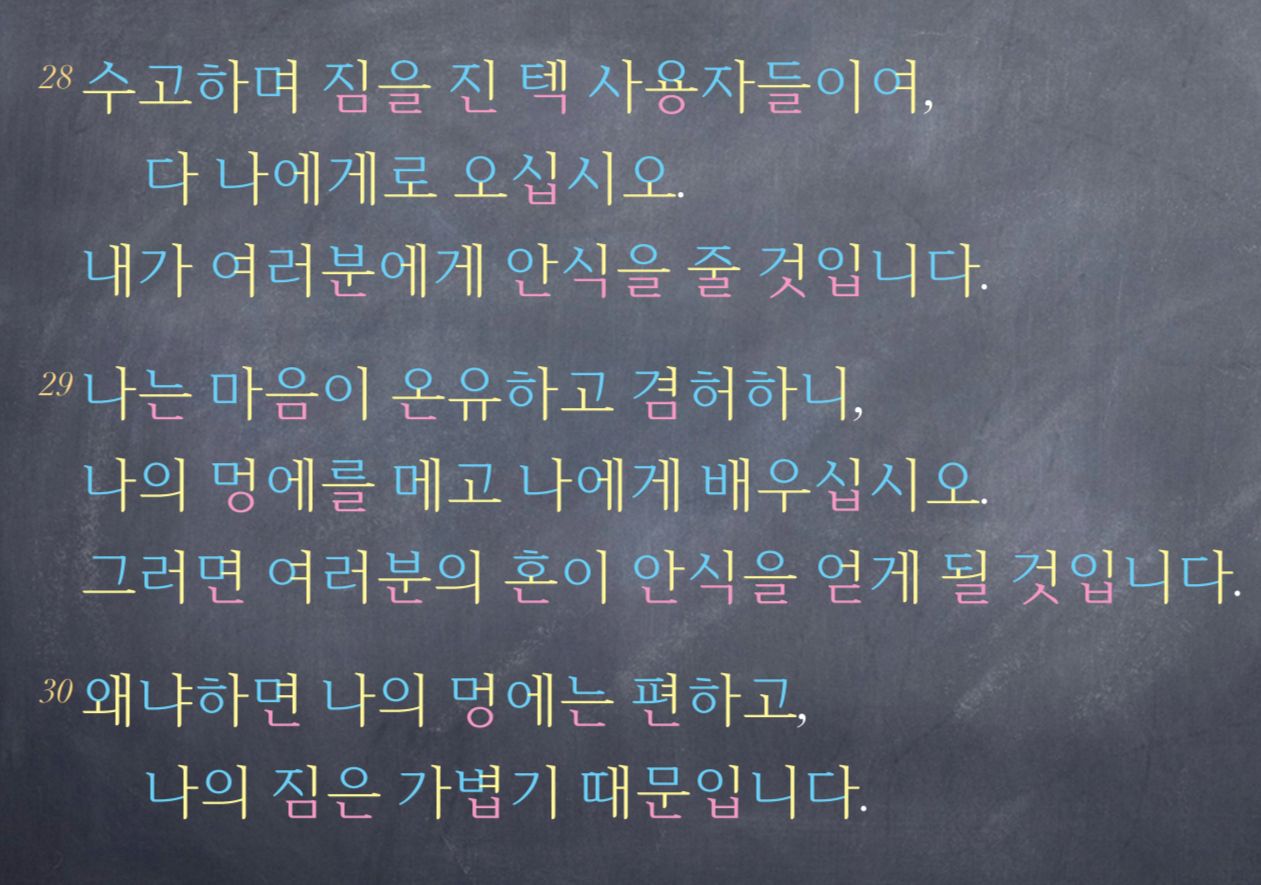
\includegraphics[width=\textwidth]{figures/cho.png}
  \end{center}
  \raggedleft\tiny\color{50gray} Jin-Hwan Cho
``A case study on TEX’s superior power: Giving different colors to building blocks of Korean syllables'' TUG 2013
  \url{http://ftp.tug.org/tug2013/slides/Cho-TUG2013Handout.pdf}より
    \end{column}
  \end{columns}
\end{frame}

\begin{frame}[t]{SCAlleSnowman}
  \sffamily
  \begin{columns}[t]
    \begin{column}{.5\textwidth}
  \begin{itemize}
\item ZR氏プロダクト
\item scsnowmanパッケージの出力をU+2603およびU+26C4のグリフとしてフォント化
\item スタイリスティックセットでマフラーの色を8種類から選べるようにしているっぽい
  \end{itemize}
    \end{column}
    \begin{column}{.5\textwidth}
  \begin{center}
    
\includegraphics[width=\textwidth]{figures/sallesnowmen.jpg}
  \end{center}
  \raggedleft\tiny\color{50gray} Takayuki YATO
``SCAlleSnowman'' 2016
  \url{https://github.com/zr-tex8r/SCAlleSnowman}より
    \end{column}
  \end{columns}
\end{frame}

\end{document}





